\chapter{Разработка алгоритмов и средств динамической идентификации}
%TODO
 
\section{Описание исследуемого объекта}
%TODO: Добавить описание котельного агрегата, базы данных

\section{Выбор архитектуры нейронных сетей}

Появление методов глубокого обучения привели к появлекнию множества различных архитектур нейронных сетей, в частности их компонентов. Архитектура нейронной сети во многом определяется классом задачи и её правильный выбор необходимо делать исходя из особенностей данных и желаемого результата. Несмотря на широкий спектр задач, которые решают те или иные архитектуры, не все модели подходят для решения задач идентификации.

\subsection{Полносвязная нейронная сеть}

Полносвязанные нейронные сети — это нейронные сети, в которых каждый 
нейрон передает свой выходной сигнал остальным нейронам, в том числе 
и самому себе. 

\begin{figure}[H]
  \centering
    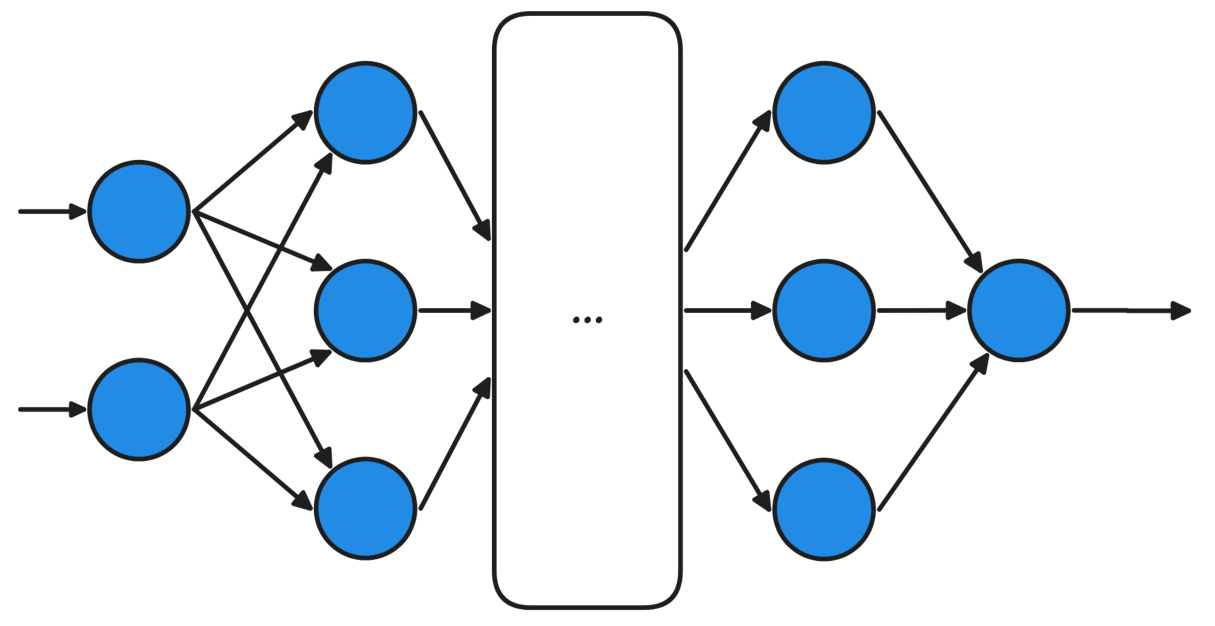
\includegraphics[width=0.9\textwidth]{figures/arch_fully_connected.png}
  \caption{Архитектура полносвязной сети}\label{fig:dense_nn}
\end{figure}

Все входные сигналы подаются всем нейронам, находящимся 
на текущем слое (см. рис. \ref{fig:dense_nn}). Выходными сигналами сети могут быть все или некоторые
выходные сигналы нейронов.

Такие модели могут использоваться для аппроксимации сложных многомерных
функций, представляющих множество целей оптимизации. Часто применяются для
построения суррогатных моделей для оценки функций без необходимости прямого
вычисления.

\subsection{Рекуррентная нейронная сеть}

Рекуррентная нейронная сеть — это тип искусственных нейронных сетей, широко
используемый для обработки последовательных данных и временных рядов. 

\begin{figure}[H]
  \centering
    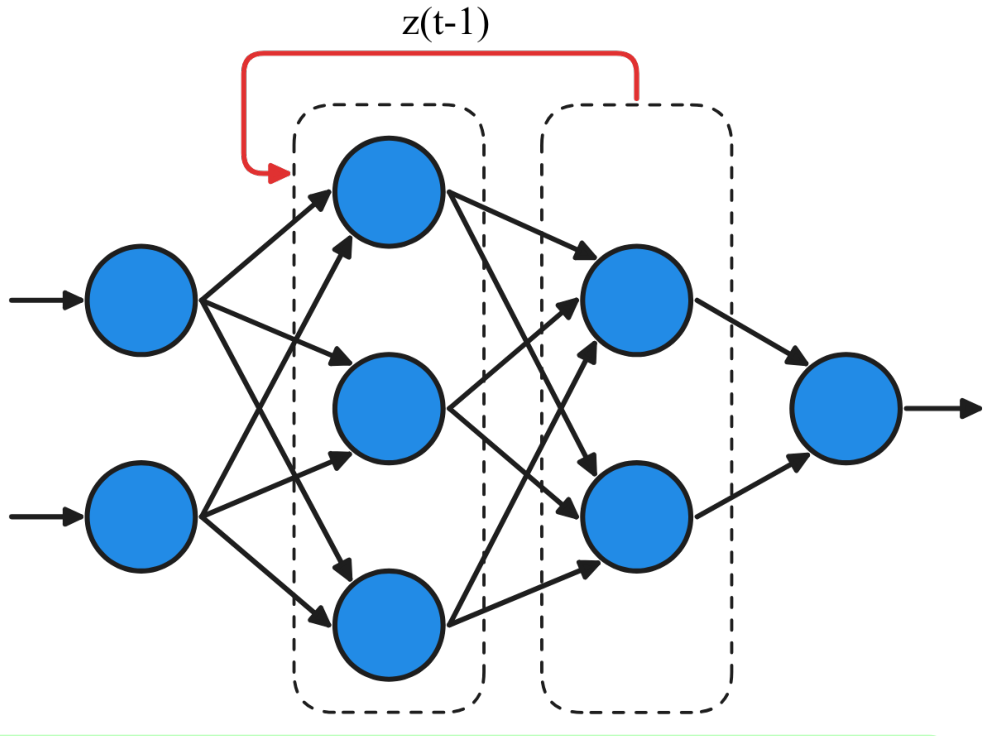
\includegraphics[width=0.9\textwidth]{figures/arch_rnn.png}
  \caption{Архитектура рекуррентной сети}\label{fig:rnn}
\end{figure}

В отличие от традиционных нейронных сетей, например, многослойных перцептронов, где
обработка данных происходит только в одном направлении, RNN имеют петли (см.
рис. \ref{fig:rnn}). Эти петли позволяют сохранять и использовать информацию из 
предыдущих состояний сети, что делает RNN особенно полезными для задач, где важен 
контекст и зависимость данных во времени. 

В задачах динамической идентификации, где необходимо учитывать не только прямые
связи систем, но также и краевые эффекты, оказывающие влияние на смежные
системы, RNN могут быть полезны благодаря своей способности учитывать контекст
и исторические данные.

\subsection{Сверточная нейронная сеть}

Сверточная нейронная сеть — особый тип нейронной сети, основанный на
полносвязной сети и имеющий как минимум один особый сверточный слой. 

\begin{figure}[H]
  \centering
    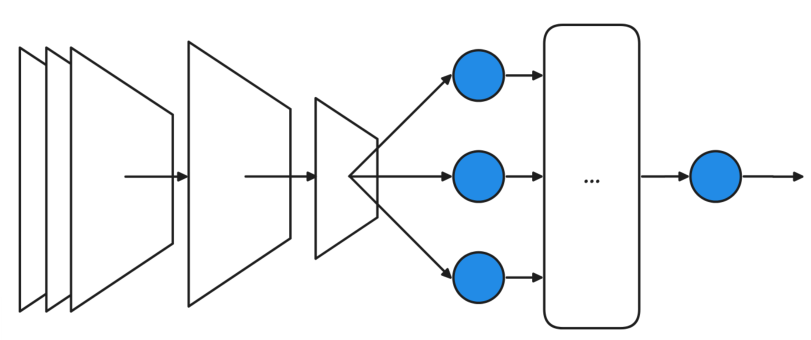
\includegraphics[width=0.9\textwidth]{figures/arch_cnn.png}
  \caption{Архитектура сверточной сети}\label{fig:cnn}
\end{figure}

Сверточный слой — нейронный слой, позволяющий производить понижение или повышение
размерности данных. Из-за своей особой архитектуры (см. рис. \ref{fig:cnn}),
сети позволяют эффективно обрабатывать данные с пространственной структурой.

Данная категория нейронных сетей применяется в случаях, если входы системы
имеют пространственную структуру, в которой элементы связанны между собой. Они
применяются для обнаружения признаков или шаблонов, влияющих на общую работу
системы.

Зачастую данный тип нейронных сетей используется в связи с другими
архитектурами, предоставляя им возможности работы с небольшими данными с
выделенными общими признаками.

\subsection{Автокодировочная нейронная сеть}

Автокодировщик — это тип нейронной сети, используемой для обучения эффективного
кодирования данных. Цель автокодировщика — научиться представлять входные
данные в более сжатом и информативном виде, называемом латентным пространством,
и затем восстанавливать оригинальные данные из этого представления. 
\begin{figure}[H]
  \centering
    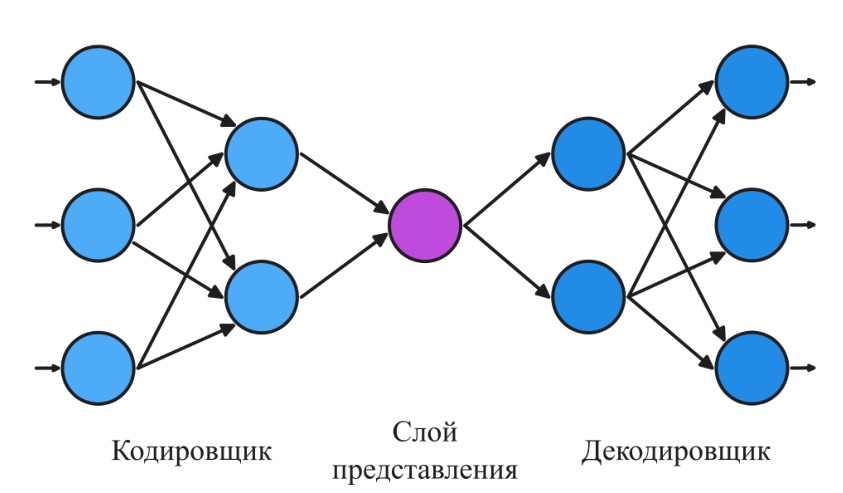
\includegraphics[width=0.9\textwidth]{figures/arch_autoencoder.png}
  \caption{Архитектура сети-автокодировщика}\label{fig:autoencoder}
\end{figure}

Он состоит из двух основных частей: энкодера и декодера (см. рис.
\ref{fig:autoencoder}). Энкодер преобразует входные данные в сжатое 
скрытое представление (латентное пространство), а декодер восстанавливает 
исходные данные из этого представления. Задача декодера — восстановить данные 
из их скрытого сжатого представления. Данный тип моделей позволяет находить 
компактные представления данных и выявлять скрытые закономерности в них.
В некоторых типах автокодировщиков добавляют вероятностную интерпретацию, что
позволяет моделировать неопределенности в данных и оптимизировать несколько
целей одновременно через латентное пространство.

Архитектурные особенности автокодировщиков не предполагают использования их в
качестве моделей, описывающих системы, однако могут использоваться с целью
повторения помех в данных и приближения их к реальным.

\subsection{Сравнение архитектур}
%TODO: Описание тестового набора

Для того, чтобы сравнить производительность различных архитектур нейронных
сетей выберем из рассмотренного ранее набора данных набор связанных параметров
и произведем для выбранной подсистемы построение цифрового двойника. 

В качестве исследуемых параметров выберем систему с одним входным и выходным
параметром - нагревательный котел. В качестве входного параметра выберем
массовый расход мазута, а выходным температура в котле. Соответственно,
повышение мазута, поступающего на нагрев котла, должно приводить к повышению
температуры внутри котла. 

\begin{figure}[H]
  \centering
    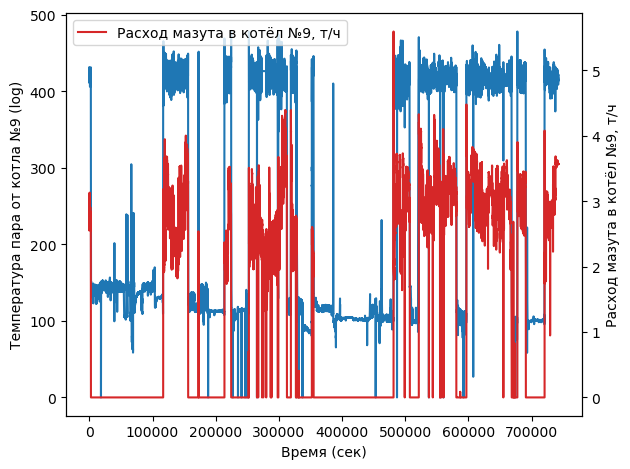
\includegraphics[width=0.85\textwidth]{figures/plots/kotel_temp_mazut.png}
  \caption{Временные характеристики параметров котла}\label{fig:plt:kotel}
\end{figure}

Из временных зависимости входного и выходного параметров (см. рис.
\ref{fig:plt:kotel}) видно, что параметры имеют связь. 

\begin{figure}[H]
  \begin{center}
    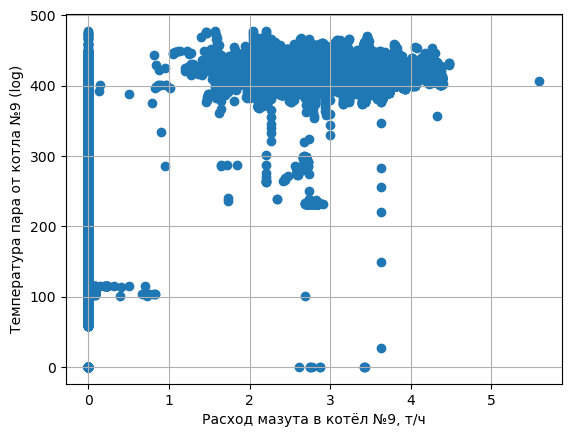
\includegraphics[width=0.85\textwidth]{figures/plots/kotel_temp_mazut_rel.png}
  \end{center}
  \caption{Корреляция между параметрами котла}\label{fig:plt:kotel:rel}
\end{figure}

Из построения характеристики между параметрами (см. рис.
\ref{fig:plt:kotel:rel}) видно, что характер зависимости не является
линейным и трудно описываем простыми выражениями. 

\subsubsection{Полносвязная сеть}

Произведем идентификацию с помощью многослойной
нейронной сети. 

\begin{figure}[H]
  \begin{center}
    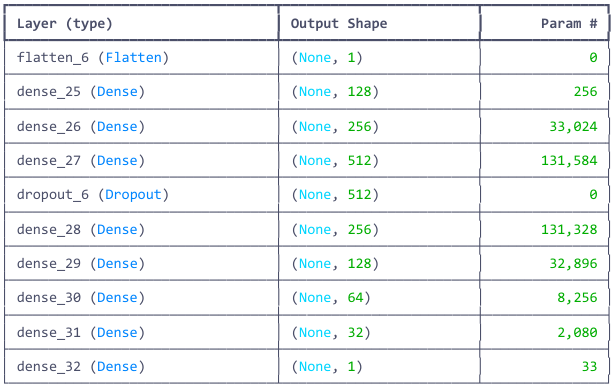
\includegraphics[width=0.95\textwidth]{figures/tensorflow/dense.png}
  \end{center}
  \caption{Конфигурация полносвязной сети}\label{fig:tf:dense}
\end{figure}

Архитектура сети выбрана исходя условия отсутствия
сужений относительно количества входов и выходов (см.
рис. \ref{fig:tf:dense}). 

Обучение производится на 50 эпохах с учетом
разделения данных на $80\%$ на обучающую выборку и
$20\%$ тестирование и валидацию. 

\begin{figure}[H]
  \begin{center}
    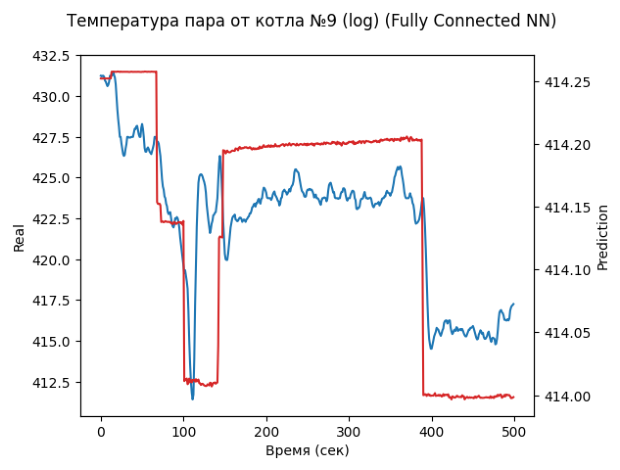
\includegraphics[width=0.95\textwidth]{figures/tensorflow/dense_compare.png}
  \end{center}
  \caption{Сравнение полученной модели полносвязной нейронной сетью}\label{fig:tf:cmp:dense}
\end{figure}

Из полученных результатов (см. рис. \ref{fig:tf:cmp:dense}) можно видеть, что
общая динамика системы повторяется, кроме того, нейтрализуются всплески,
обусловленные шумом. 

\subsubsection{Рекуррентная сеть}

Произведем идентификацию с помощью рекуррентной
нейронной сети. 

\begin{figure}[H]
  \begin{center}
    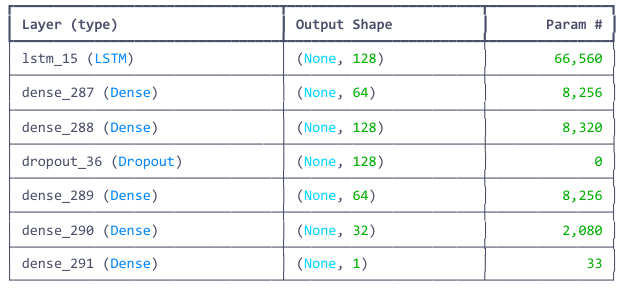
\includegraphics[width=0.95\textwidth]{figures/tensorflow/rnn.png}
  \end{center}
  \caption{Конфигурация рекуррентной сети}\label{fig:tf:rnn}
\end{figure}

Архитектура сети выбрана исходя условия отсутствия
сужений относительно количества входов и выходов (см.
рис. \ref{fig:tf:rnn}). 

Обучение будем производить с теми же свойствами, что и предыдущую. 

\begin{figure}[H]
  \begin{center}
    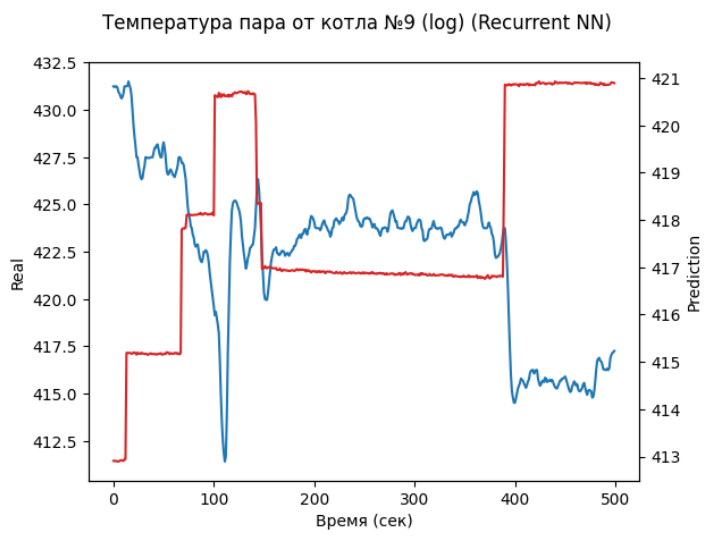
\includegraphics[width=0.95\textwidth]{figures/tensorflow/rnn_compare.png}
  \end{center}
  \caption{Сравнение полученной модели рекуррентной нейронной
  сетью}\label{fig:tf:cmp:rnn}
\end{figure}

Из полученных результатов (см. рис. \ref{fig:tf:cmp:rnn}) можно видеть, что
общая динамика системы повторяется, кроме того, нейтрализуются всплески,
обусловленные шумом, однако выход сети перевернут. 

\begin{figure}[H]
  \begin{center}
    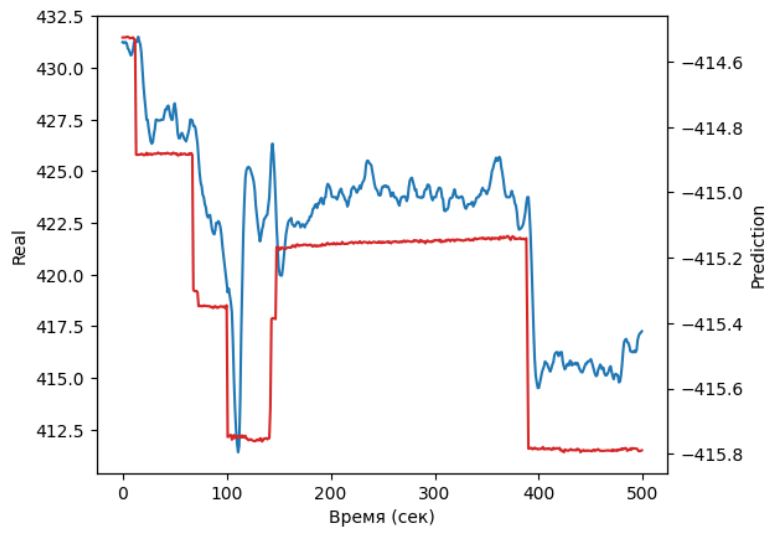
\includegraphics[width=0.95\textwidth]{figures/tensorflow/rnn_compare_reversed.png}
  \end{center}
  \caption{Сравнение полученной модели рекуррентной нейронной
  сетью}\label{fig:tf:cmp:rnn:reversed}
\end{figure}

С учетом переворота графика получаем, что метод имеет меньшую статическую
ошибку нежели полносвязная сеть (см. рис. \ref{fig:tf:cmp:rnn:reversed}).

Однако, реккурентная сеть позволяет получать только следующие значения,
основываясь на последовательностях. Для идентификации, основывающейся на
фактических параметрах модели лучшен использовать полносвязную сеть, наиболее подробно повторяющую динамику системы. 

\section{Декомпозиционный метод идентификации нейронными сетями}
%TODO: Описание предлагаемого метода
Большинство методов идентификации предполагают создание общей модели в виде
<<черного ящика>>, однако для многих больших систем такое моделирование, в
случае наличия дополнительных данных о внутренних сигналах, может быть
неэффективно. Причиной для этого может служить упущением данных о внутренней
структуре или подсистемах, взаимодействующих друг с другом и оказывающих
влияние на общий результат. Кроме того, зачастую необходимо учитывать значение
параметров подсистем при определенных режимах работы.

Точность идентификации во многом зависит от сложности рассматриваемой системы.
Малые системы дают более точный результат при меньшей сложности создания модели
или обучении нейронной сети. Из этого можно сделать вывод, что точность
построения цифрового двойника во многом связана с размером моделируемой
системы, чем меньше система, тем проще её описать. 

В связи с этим, предлагается непараметрический метод идентификации с
использованием связанного множества нейронных сетей, представляющих подсистемы
общей системы. Каждая рассматриваемая нейронная сеть иммитирует поведение
каждой своей подсистемы. При этом всём важно обеспечить связь между
подсистемами для моделирования все системы в целом. Для этого необходимо
соотвествтующее программное обеспечение, которое бы позволяло производить
полный цикл действий по динамической идентификации предложенным методом. 

\section{Программное обеспечение динамической идентификации}
%TODO: Привести информацию о наличии других ПО для моделирования
%       и то, что зачастую сложные методы поставляются с использованием замкнутого цикла ПО

Разработка удобного графического интерфейса, наиболее полно расрывающего
возможности предлагаемого решения для пользователья, сложный процесс, требующий
точного и скурпулёзного проектирования. В рамках разработки важными этапами
являются:

\begin{itemize}
  \item Выделение требований к разрабатываемой системе;
  \item Определение паттернов и структур данных;
  \item Реализация интерфейса;
  \item Оценка работы системы.
\end{itemize}

\subsection{Требования к системе}
%TODO: Привести требования к предлагаемому ПО

Выделение требований один из наиважнейших этапов, который выделяет необходимые требования и возможности будущего приложения. В рамках разработки приложения для реализации предложенного метода идентификации были выделены следующие требования:

\begin{itemize}
  \item Создавать или загружать данные о сигналах;
  \item Конфигурировать системы с заданным именем, входными и выходными
    сигналами;
  \item Объединять созданные подсистемы в единую связанную систему в
    соответствии с параметрами, определенными пользователем;
  \item Задавать параметры обучения для каждой системы;
  \item Отображать созданную систему в виде связанного графа;
  \item Позволять вручную вводить значения для каждого из сигналов;
  \item Сохранять параметры систем и их иерархию в виде файлов.
\end{itemize}

Все выше перечисленные возможности должны быть реализованы в рамках одного приложения.


\subsection{Структуры данных}
%TODO: Какие структуры данных, их иерархия, паттерны использовались
Основой любого приложения являются данные. Правильный выбор абстракций и определение необходимых структур данных на начальном этапе разработке играет большую роль, определяющую такие свойства приложения как масштабируемость приложения с возможностью расширения функциональных возможностей. 

Кроме того, важно выбрать паттерны проектирования, позволяющие работать с большим количеством объектов. 

В рамках анализа базовых компонентов было выделено 2 основных базовых класса: 

\begin{itemize}
  \item Связь (Connection);
  \item Система (System). 
\end{itemize}

\subsubsection{Класс <<Связь>>}

Класс связи (Connection) предназначен для реализации связывания подсистем и процессов, протекающих между системами. 

Класс также обеспечивает возможности передачи сведений от одной системы к другой (значений сигналов). 

Каждый сигнал уникален и не повторяет по имени никакой другой.

\subsubsection{Класс <<Система>>}

Класс системы (System) предназначен для абстракции данных, связанных с
какой-либо подсистемой. Он содержит информацию о сигналах, являющихся входными
или выходными. Также, он содержит информацию о модели нейронной сети,
аппроксимирующей её поведение. 

Каждая система должна удовлетворять критерию уникальности и не быть дубликатом
другой системы. 

\subsubsection{Менеджеры классов}

Для корректного использования объектов систем и сигналов
реализованы классы, управляющие созданием и изменением объектов данного
класса – менеджеры. 

Каждый класс-менеджер, ConnectionManager и SystemManager, реализует паттерны
Singleton и Abstract Factory - в рамках всего приложения менеджеры уникальны и
учитывают созданные в текущей сессии системы и связи. 

Также, менеджеры обеспечивают учет связей между компонентами, помня какой
сигнал с какой системой связан, позволяя получать граф связей без необходимости
обхода всей системы.

\subsubsection{Вспомогательные классы}

Для поддержания абстракций реализован класс аппроксиматор, реализуйющий
создание и обучение нейронной сети для конкретной заданной системы -
SystemNeuralModel. Любые действия, связанные с идентификационной моделью,
включая создание, обучение или моделирование, выполняется через него. 

\begin{figure}[H]
  \begin{center}
    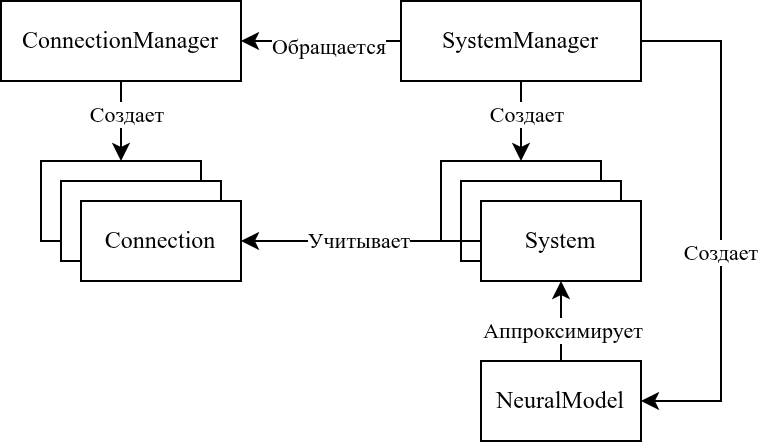
\includegraphics[width=0.95\textwidth]{figures/basics_relations.png}
  \end{center}
  \caption{Взаимодействие базовых компонент системы}\label{fig:basics:components}
\end{figure}

Каждый из классов (см. рис. \ref{fig:basics:components}) работает в связи с другими и реализует базовый функционал для конфигурации исследуемых сигналов и систем.

\subsection{Архитектура приложения}
%TODO: Привести список компонентов, их назначение и связь между собой

\begin{figure}[H]
  \begin{center}
    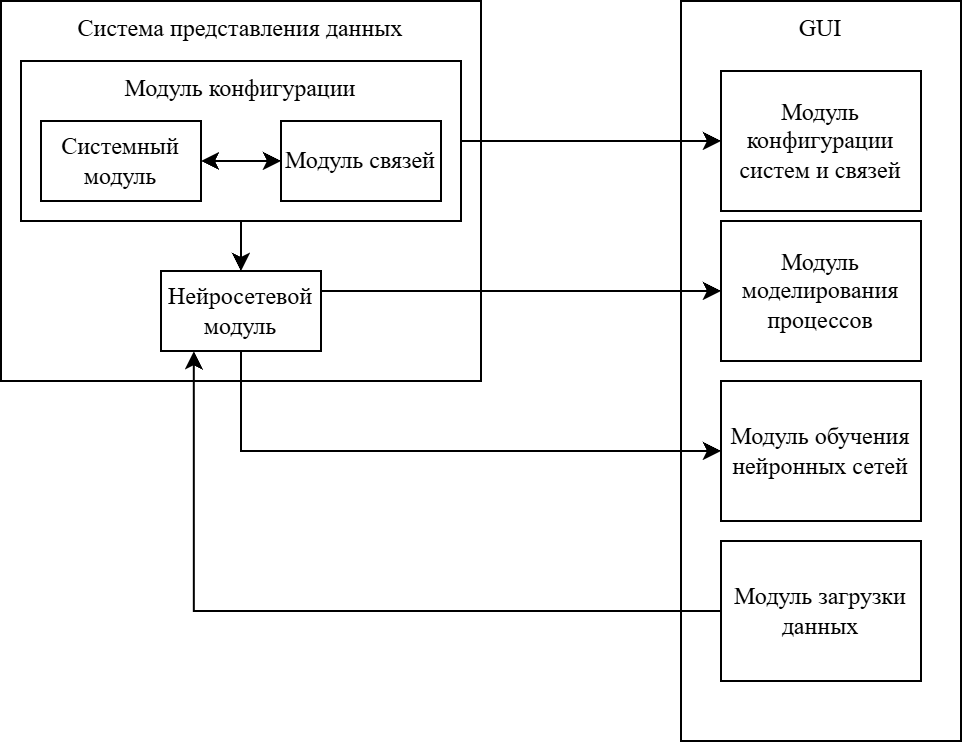
\includegraphics[width=0.95\textwidth]{figures/modules/relations.png}
  \end{center}
  \caption{Модульные связи приложения}\label{fig:modules:relation}
\end{figure}


\subsection{Используемые формы}
%TODO: Перечисление форм и их назначение, какие возможности предоставляют

\begin{figure}[H]
  \begin{center}
    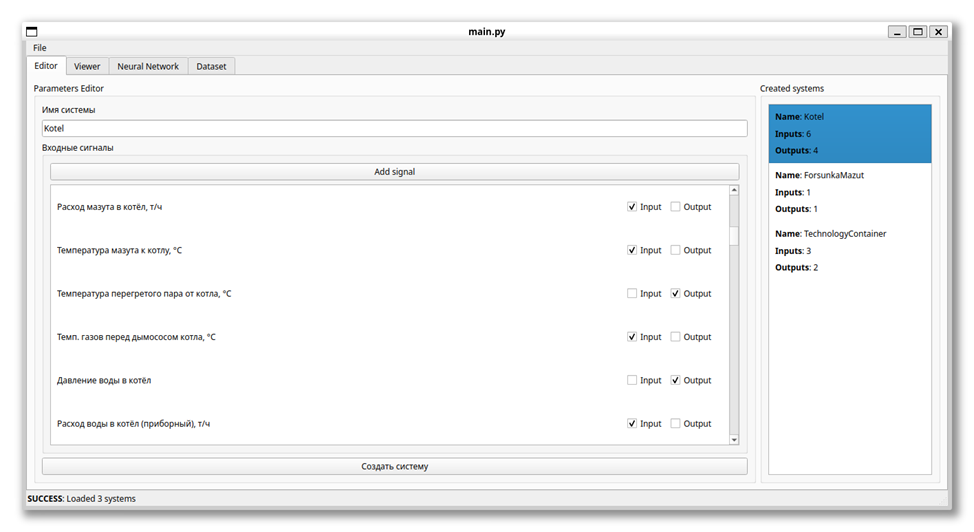
\includegraphics[width=0.95\textwidth]{figures/modules/editor.png}
  \end{center}
  \caption{Форма конфигурации систем и связей}\label{fig:forms:editor}
\end{figure}

\begin{figure}[H]
  \begin{center}
    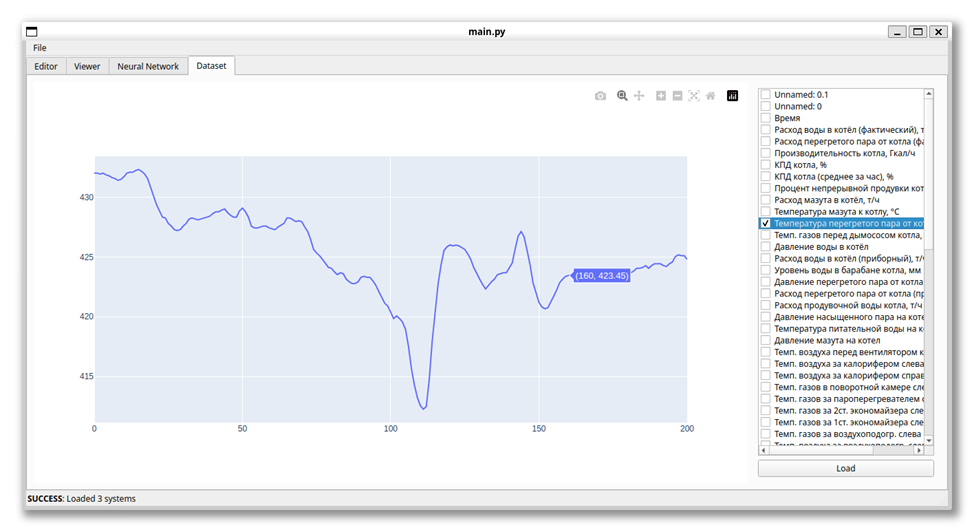
\includegraphics[width=0.95\textwidth]{figures/modules/loader.png}
  \end{center}
  \caption{Форма загрузки и обработки данных}\label{fig:forms:loader}
\end{figure}


\begin{figure}[H]
  \begin{center}
    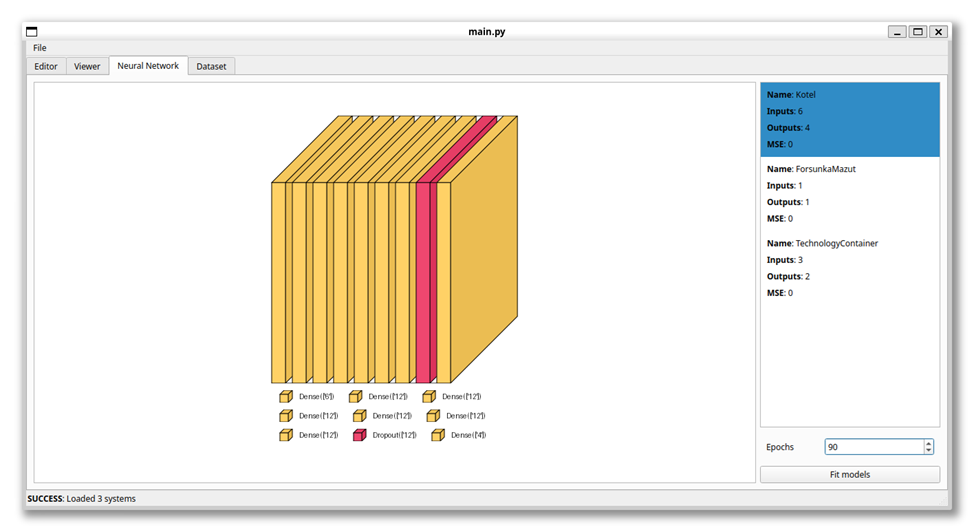
\includegraphics[width=0.95\textwidth]{figures/modules/neural.png}
  \end{center}
  \caption{Форма настройки обучения и структуры нейронных сетей}\label{fig:forms:neural}
\end{figure}

\begin{figure}[H]
  \begin{center}
    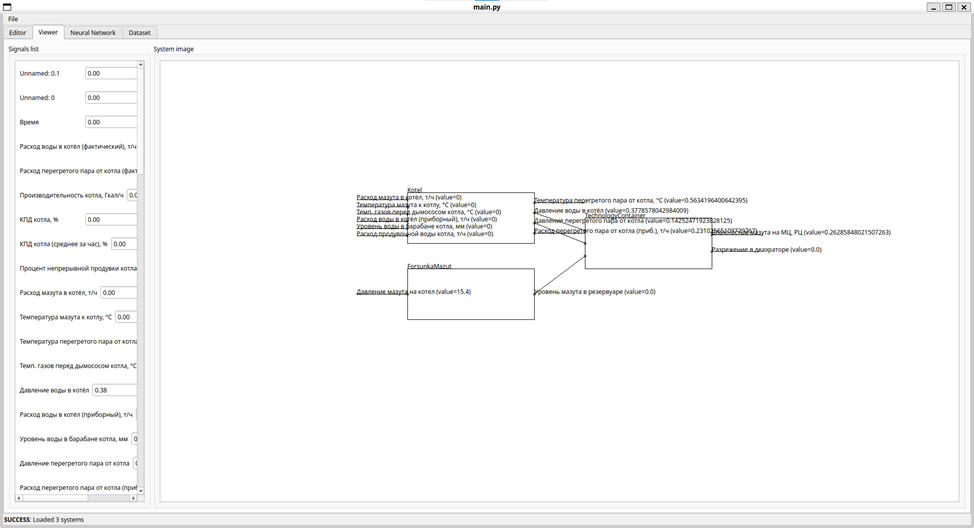
\includegraphics[width=0.95\textwidth]{figures/modules/modelling.png}
  \end{center}
  \caption{Форма загрузки и обработки данных}\label{fig:forms:viewer}
\end{figure}

\subsection{Работа с приложением}
%TODO: Описать как работать с приложением и какие возможности оно предоставляет

\section{Архитектура связей нейронных сетей}
%TODO: Описать какие модели используются при обучении для описания каждой подсистемы и системы в общем

\section{Оценка работы}
%TODO: Произвести оценку моделирования системы
